\documentclass{amsart}

%%%%%%%%%%%%%%%%%%%%%%%%%%%%%%%%%%%%%%

\usepackage[utf8]{inputenc}
\usepackage[T1]{fontenc}

\usepackage{a4wide}%en grand
\usepackage{changepage}%indentation

\usepackage{xcolor}
\usepackage{amsfonts,amsthm,amssymb,amsmath}
\usepackage{mathtools}
\usepackage{wasysym}
\usepackage{xspace}
\usepackage{graphicx}
\usepackage[notcite,notref]{showkeys} % shows labels 
\usepackage{breqn}
\usepackage{algorithm}
\usepackage{algorithmic}
\usepackage{tabularx}

\usepackage[english]{babel} %gestion des langues
\usepackage{caption}
\usepackage{subcaption}
\usepackage{paralist}
\usepackage{multirow}

\usepackage{hyperref}
\hypersetup{colorlinks=true, citecolor=darkblue, linkcolor=darkblue}
\usepackage{hypcap}

\usepackage[noabbrev,capitalise]{cleveref}
\usepackage{autonum}
\usepackage{xspace}

%%%%%%%%%%%%%%%%%%%%%%%%%%%%%%%%%%%%%%

\newtheorem{theorem}{Theorem}[section]
\newtheorem{proposition}[theorem]{Proposition}
\newtheorem{lemma}[theorem]{Lemma}
\newtheorem{ce}[theorem]{Counter-example}
\newtheorem{claim}[theorem]{Claim}
\newtheorem{corollary}[theorem]{Corollary}
\newtheorem{definition}[theorem]{Definition}
\newtheorem{notation}[theorem]{Notation}
\theoremstyle{remark}
\newtheorem{remark}{Remark}[section]
\newtheorem{example}{Example}
\newtheorem{algo}{Algorithm}
\newtheorem*{example*}{Example}

\crefname{theorem}{Theorem}{Theorems}
\crefname{lemma}{Lemma}{Lemmas}

\definecolor{darkblue}{rgb}{0,0,0.7} % darkblue color
\newcommand{\darkblue}{\color{darkblue}} % darkblue command
\newcommand{\defn}[1]{\textsl{\darkblue #1}} % emphasis of a definition

%%%%%%%%%%%%%%%%%%%%%%%%%%%%%%%%%%%%%%

% math special letters
\newcommand{\R}{\mathbb{R}} % reals
\newcommand{\N}{\mathbb{N}} % naturals
\newcommand{\Z}{\mathbb{Z}} % integers
\newcommand{\C}{\mathbb{C}} % complex

% math commands
\newcommand{\set}[2]{\left\{ #1 \;\middle|\; #2 \right\}} % set notation
\newcommand{\bigset}[2]{\big\{ #1 \;\big|\; #2 \big\}} % big set notation
\newcommand{\Bigset}[2]{\Big\{ #1 \;\Big|\; #2 \Big\}} % Big set notation
\newcommand{\setangle}[2]{\left\langle #1 \;\middle|\; #2 \right\rangle} % set notation
\newcommand{\ssm}{\smallsetminus} % small set minus
\newcommand{\dotprod}[2]{\left\langle \, #1 \; \middle| \; #2 \, \right\rangle} % dot product
\newcommand{\symdif}{\,\triangle\,} % symmetric difference
\newcommand{\one}{{1\!\!1}} % the all one vector
\newcommand{\eqdef}{\mbox{\,\raisebox{0.2ex}{\scriptsize\ensuremath{\mathrm:}}\ensuremath{=}\,}} % :=
\newcommand{\defeq}{\mbox{~\ensuremath{=}\raisebox{0.2ex}{\scriptsize\ensuremath{\mathrm:}} }} % =:
\newcommand{\viceversa}{\textit{vice versa}} % vice versa

\newcommand*{\dual}[1]{{#1^*}}
\newcommand*{\nbd}[0]{neighbourhood\xspace}
\newcommand*{\ef}[0]{E-finite\xspace}
\newcommand*{\vf}[0]{V-finite\xspace}
\newcommand*{\ktg}[0]{$k$-triangulation\xspace}

\newcommand{\cl}{\prec}
\newcommand{\cle}{\preccurlyeq}

\newcommand{\surface}{\mathcal{S}}
\newcommand{\cylinder}{\mathcal{C}}

\graphicspath{{../figures/}}

% marginal comments
\usepackage{todonotes}
\newcommand{\vincent}[1]{\todo[color=blue!30]{#1 \\ \hfill --- V.}}
\newcommand{\mathias}[1]{\todo[color=red!30]{#1 \\ \hfill --- M.}}

%%%%%%%%%%%%%%%%%%%%%%%%%%%%%%%%%%%%%%

\title[Infinite multitriangulations and multitriangulations of surfaces]{Infinite multitriangulations \\ and multitriangulations of surfaces}

\thanks{ML was partially supported by the French ANR grant GATO~(16\,CE40\,0009). \\ \indent VP was partially supported by the French ANR grants SC3A~(15\,CE40\,0004\,01) and CAPPS~(17\,CE40\,0018).}

\author{Mathias Lepoutre}
\address{LIX, \'Ecole Polytechnique, Palaiseau}
\email{mathias.lepoutre@lix.polytechnique.fr}
\urladdr{\url{http://www.lix.polytechnique.fr/Labo/Mathias.Lepoutre/}}

\author{Vincent Pilaud}
\address{CNRS \& LIX, \'Ecole Polytechnique, Palaiseau}
\email{vincent.pilaud@lix.polytechnique.fr}
\urladdr{\url{http://www.lix.polytechnique.fr/~pilaud/}}

%%%%%%%%%%%%%%%%%%%%%%%%%%%%%%%%%%%%%%

\begin{document}

\begin{abstract}
We extend previous work on the structure of $k$-stars of a multi-triangulation on a convex polygon to the case of multi-triangulations on any surface, orientable or not. 

To that extent, we use the universal cover construction, that makes a map on a surface into a periodic map of an infinite polygon. We generalize the work of Pilaud and Santos to multi-triangulation of an infinite polygon, with some additional constraints, and then conclude about the case of multi-triangulations on any surface.
\end{abstract}

\maketitle

\begin{figure}[h]
	\capstart
	\centerline{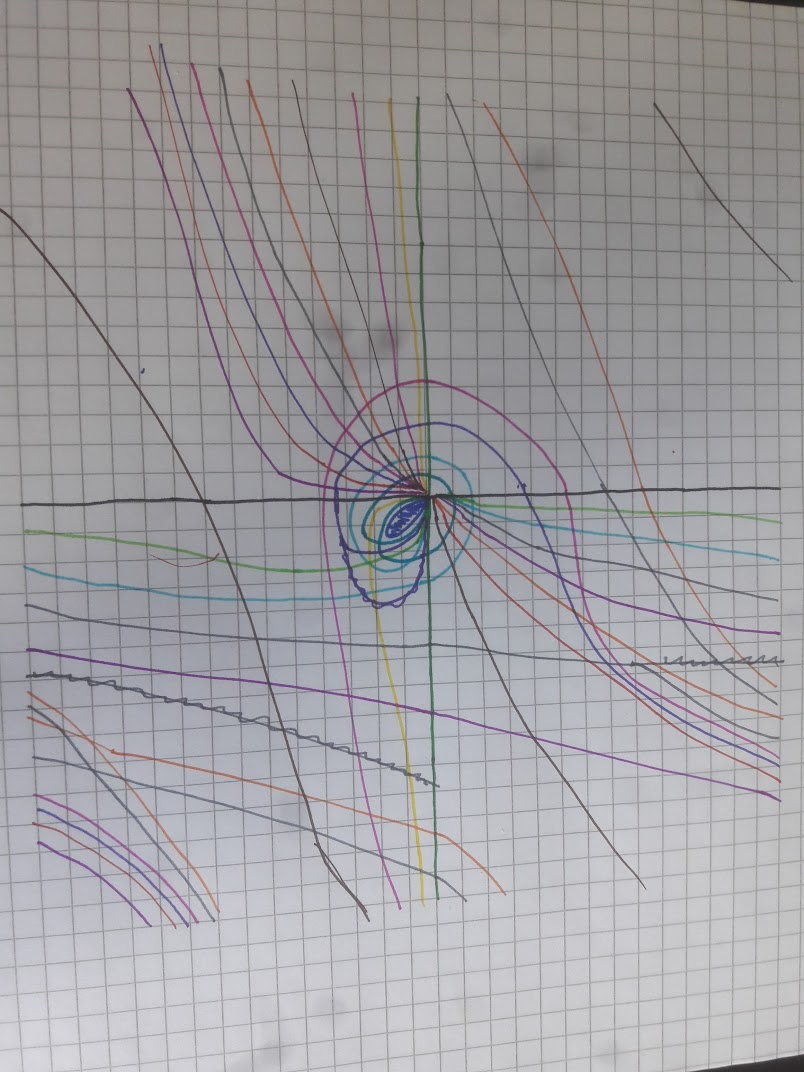
\includegraphics[scale=.42]{torus}}
	\caption{The universal cover of the $2$-triangulation of a torus with a hole, represented in \cref{fig:torus}}
	\label{fig:UCtorus}
\end{figure}

%%%%%%%%%%%%%%%%%%%%%%%%%%%%%%%%%%%%%%

\section{Multitriangulations of infinite polygons}
\label{sec:infiniteMultitriangulations}

%%%%%%%%%%%%

\subsection{Infinite polygons}

\begin{definition}
A \defn{polygon}~$P$ is a cyclically ordered set, that might be finite or infinite.
We write~$a \cl b \cl c$ for the cyclic order.
The elements of~$P$ are called \defn{points} and pairs of elements of~$P$ are called \defn{diagonals}.
For two points~$a,b \in P$, let~$[a,b] \eqdef \set{c \in P}{a \le c \le b}$, and define similarly the intervals~$[a,b[$, $]a,b]$ and~$]a,b[$ (with open brackets for strict inequalitites).
Two diagonals~$(a,c)$ and~$(b,d)$ of~$P$ \defn{cross} if~$a \cl b \cl c \cl d$.
\end{definition}

\begin{definition}
If $x$ and $y$ are two points of a polygon~$P$ such that the interval~$]x,y[$ is empty, we say that~$x$ is the \defn{predecessor} of~$y$ and that~$y$ is the \defn{successor} of~$x$, and we use the notations~$y = x+1$ and~$x = y-1$. A polygon~$P$ is \defn{tidy} if each point of~$P$ has both a predecessor and a successor. In particular, finite polygons are tidy.
\end{definition}

\begin{definition}
A set~$X$ of diagonals of a polygon~$P$ is 
\begin{itemize}
\item \defn{\ef} if each diagonal of~$X$ is crossed by a finite number of diagonals of~$X$,
\item \defn{\vf} if each vertex of~$P$ is incident to finitely many diagonals of~$X$.
\end{itemize}
\end{definition}

\begin{definition}[periodic]

\end{definition}

%%%%%%%%%%%%

\subsection{Infinite multitriangulations}

\begin{definition}
A \defn{$k$-crossing} of a polygon~$P$ is a set of~$k$ pairwise crossing diagonals of~$P$.
A \defn{$k$-triangulation} of~$P$ is an inclusion-maximal set of diagonals of~$P$ with no $(k+1)$-crossing.
\end{definition}

\begin{definition}
The \defn{length} of a diagonal~$(a,b)$ of a polygon~$P$ is the minimum~$\ell(a,b)$ of~$|{]a,b[}|$ and~$|{]b,a[}|$ (note that this might be infinite).
A diagonal~$(a,b)$ with~$\ell(a,b) > k$ (resp.~$\ell(a,b) = k$, resp.~$\ell(a,b) < k$) is a \defn{$k$-relevant} (resp.~\defn{$k$-boundary}, resp.~\defn{$k$-irrelevant}) diagonal.
\end{definition}

\begin{remark}
Observe that a diagonal contained in a $(k+1)$-crossing must be $k$-relevant.
Therefore, any \ktg contains all $k$-irrelevant and $k$-boundary diagonals by maximality.
\end{remark}


\begin{definition}
A \defn{$k$-star} of a polygon~$P$ is a set of diagonals of~$P$ of the form~$\set{(s_i, s_{i+k})}{0 \le i \le 2k}$ where~$s_0 \cl \dots \cl s_{2k}$ (the indices are understood modulo~$2k+1$).
\end{definition}

\begin{definition}
An \defn{angle} of a set~$X$ of diagonals of a polygon~$P$ is a pair of diagonals~$\{(u,v), (v,w)\}$ with~$u \cl v \cl w$ such that~$X$ contains no diagonal of the form~$(v,t)$ with~$w \cl t \cl u$. The angle is denoted by~$\angle(u,v,w)$ and we say that~$v$ is the \defn{apex} of~$\angle(u,v,w)$. An angle is \defn{$k$-relevant} if none of its diagonals is $k$-irrelevant. %A set~$Y$ of diagonals of~$P$ crosses the angle~$\angle(u,v,w)$ if each diagonal of~$Y$ crosses both~$(u,v)$ and~$(v,w)$. 
\end{definition}

One of the objectives of this paper is to prove the following structural results on infinite multitriangulations

\begin{theorem}
\label{thm:structureInfinite}
Let~$T$ be a \ef \ktg of a tidy polygon~$P$.
\begin{enumerate}
\item Each $k$-relevant angle of~$T$ is contained in precisely one $k$-star of~$T$.
\item Each $k$-relevant (resp.~$k$-boundary, resp.~$k$-irrelevant) diagonal of~$P$ is contained in precisely two (resp.~one, resp.~none) $k$-stars of~$T$.
\item For any $k$-relevant diagonal~$e$ of~$T$, there exists a unique diagonal~$f$ not in~$T$ such that~$T \symdif \{e,f\}$ is another $k$-triangulation. The diagonal~$f$ only depend on the two $k$-stars of~$T$ containing~$e$.
\item Let~$P'$ denote a polygon obtained by replacing $k+1$ consecutive points of~$P$ by~$k$ points. Then there exists a flattening (resp.~inflating) operation that transforms the \ktg{}s of~$P$ into the \ktg{}s of~$P'$ (resp.~and \viceversa).
\item For any point~$p$ of the plane, the $k$-depth of~$p$ in~$P$ is equal to the sum of the winding numbers around~$p$ of the $k$-stars of~$T$.
\vincent{Vrai ?}
\end{enumerate}
\end{theorem}

We prove \cref{thm:structureInfinite} (1-3) in \cref{sec:prfInfinite}.

\begin{remark}
\begin{itemize}
\item flip graph connected? Increasing flip graph?
\item duality with pseudoline arrangements?
\item $k$-arboresence? connection to $k$-edge-connected but not locally $(k+1)$-edge-connected.
\end{itemize}
\end{remark}

%%%%%%%%%%%%

\subsection{Some counter-examples}

\begin{ce}
The polygon of a periodic \ktg is not necessarily a \nbd.
\end{ce}
\begin{proof}

\end{proof}

\begin{ce}
A periodic \ef \ktg may have angles that are not crossed by a $(k-1)$-crossing.
\end{ce}
\begin{proof}

\end{proof}

\begin{ce} 
A periodic \ktg may not be \ef.
\end{ce}
\begin{proof}

\end{proof}

\begin{ce}
A \ef \ktg of a \nbd is not necessarily \vf.
\end{ce}
\begin{proof}
k=1
\end{proof}

%%%%%%%%%%%%%%%%%%%%%%%%%%%%%%%%%%%%%%

\section{Multitriangulations of a general surface}

%%%%%%%%%%%%

\subsection{definitions}

\begin{definition}
Consider a connected surface~$\surface$ with boundary and a set~$V$ of marked points on the boundary, with at least one marked point on each boundary component. An \defn{arc} of~$\surface$ is a curve on~$\surface$ connecting two points of~$V$ and whose interior is disjoint from the boundary of~$\surface$. We consider arcs up to homotopy relative to their endpoints in~$\surface$ and we disallow arcs homotopic to a boundary segment of~$\surface$.
\end{definition}
\mathias{Why should we disallow arcs homotopic to a boundary segment of~$\surface$? are they not just $k$-irrelevant diagonals of length $1$?}

\begin{remark}
We could also consider the case of a surface with no marked points on some boundaries. Be careful that the definition of $k$-relevant, $k$-boundary and $k$-irrelevant diagonals are not clear anymore in that case.
\end{remark}

\begin{definition}
Universal cover~$\pi : \bar\surface \to \surface$.
\vincent{UC Not clear}
\end{definition}

\begin{definition}
A \defn{$k$-crossing} on~$\surface$ is a collection~$\alpha_1, \dots, \alpha_k$ (possibly with repetition) of $k$ arcs of~$\surface$ which admit pairwise crossing representatives~$\bar\alpha_1, \dots, \bar\alpha_k$ in the universal cover~$\bar\surface$.
A \defn{$k$-triangulation} of~$P$ is an inclusion maximal set of diagonals of~$P$ with no $(k+1)$-crossing.
\end{definition}

\begin{remark}
Be careful: a $k$-crossing on~$\surface$ is NOT a collection of pairwise crossing arcs of~$\surface$. Namely, there are collections of pairwise crossing arcs of~$\surface$ which do not admit pairwise crossing representatives. The simplest examples are self-crossing arcs, since their representative are not self-crossing. Further examples are given in \cref{fig:notkcrossing}.
\vincent{Todo.}
\end{remark}

\begin{theorem}
\label{thm:structureSurface}
Any \ktg of a surface of genus~$g$ with~$b$ boundaries and~$n$ marked points has precisely $n + 2k(2g + b - 2)$ $k$-stars and $kn + k(2k + 1)(2g + b - 2)$ $k$-relevant arcs.
\end{theorem}


\begin{remark}
\begin{itemize}
\item \cite[Lem.~7.10]{PilaudSantos}: Any $k$-triangulation of the $n$-gon contains at most $k(n-2p-1)$ $p$-relevant diagonals. Extension for surfaces.
\item flip graph connected? Increasing flip graph? Is it a lattice? (use bracket vectors)
\item duality? Line space of the surface?
\item punctures?
\end{itemize}
\end{remark}


\begin{figure}[h]
	\capstart
	\centerline{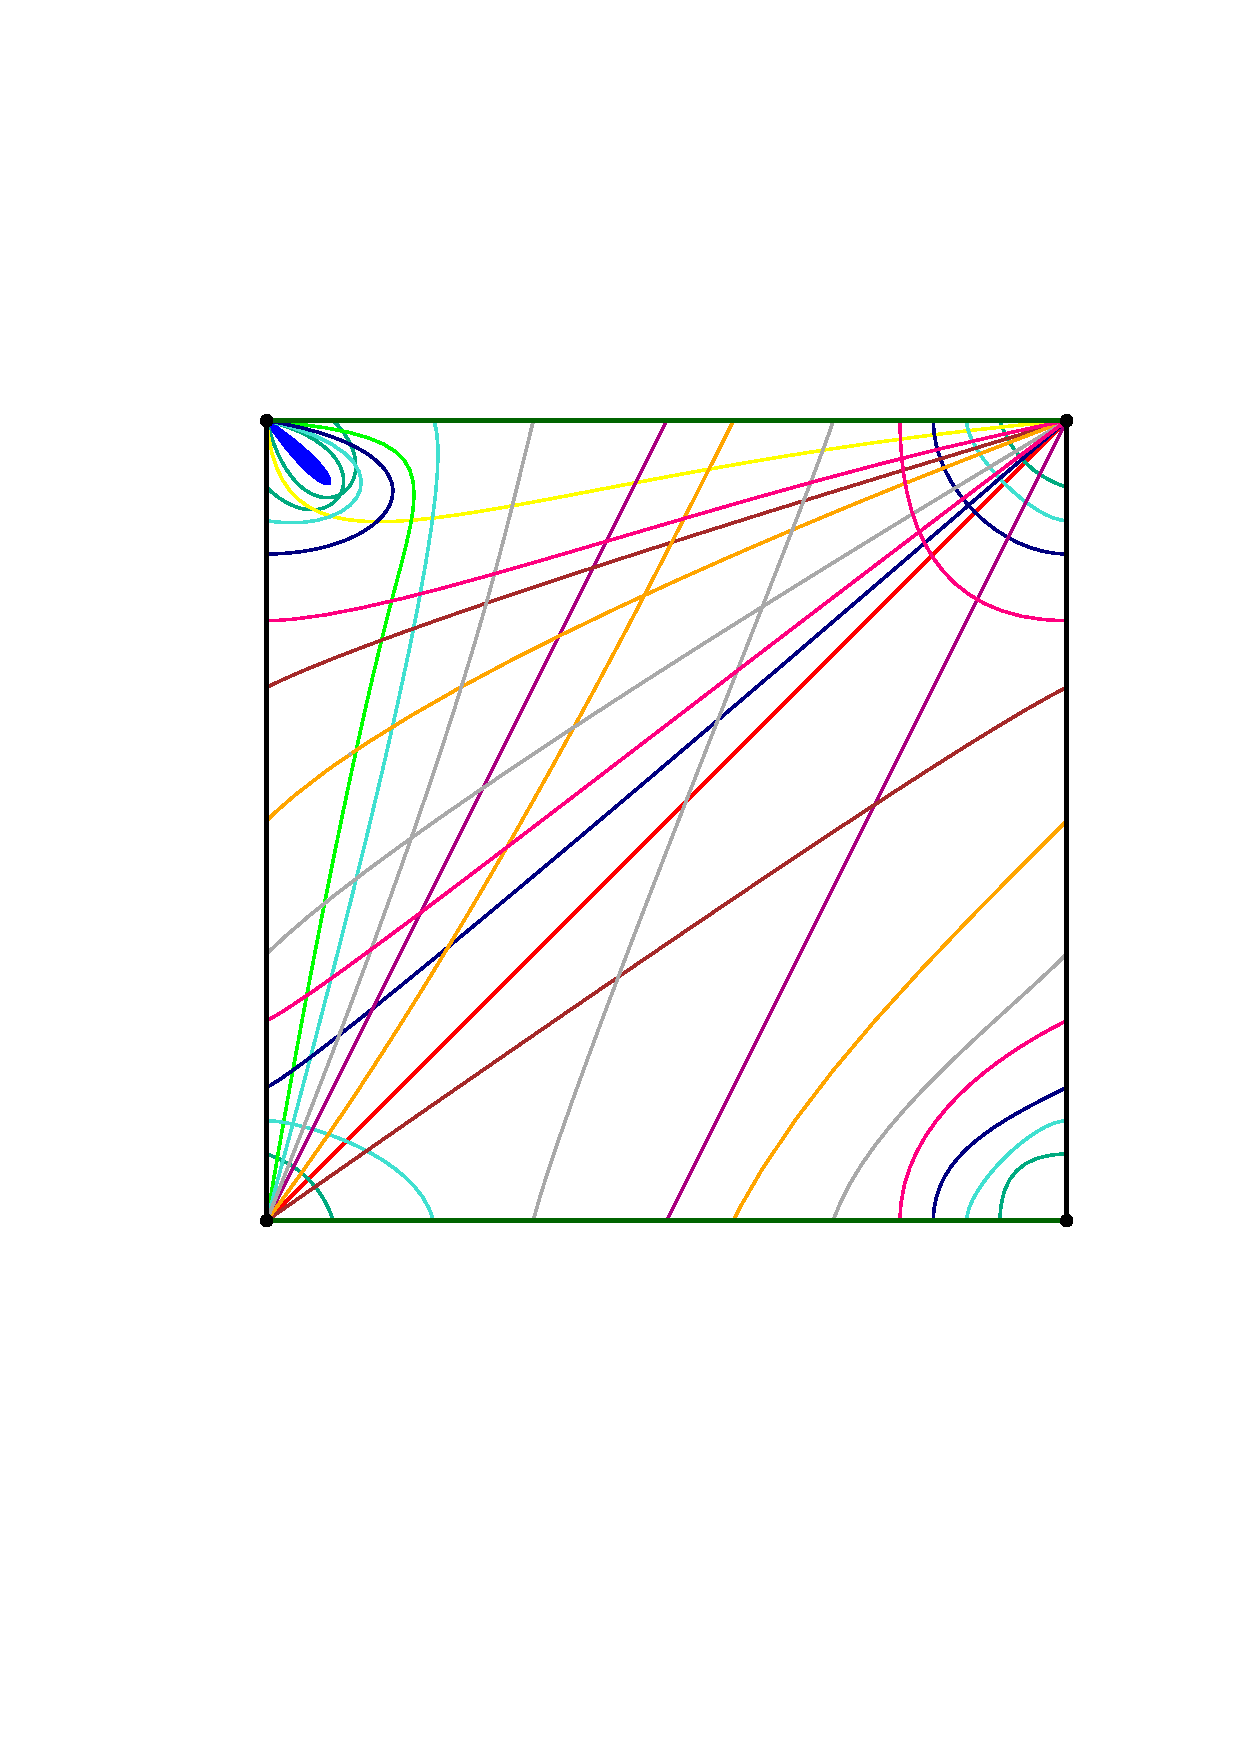
\includegraphics[scale=.42]{exTorusSquare}}
	\caption{A $2$-triangulation of a torus with a hole (in blue), whose universal cover is represented in \cref{fig:UCtorus}}
	\label{fig:torus}
\end{figure}


\begin{theorem}
\label{generalFlip}
Any $k$-relevant edge of a $k$-triangulation on a surface can be flipped.
\end{theorem}

%%%%%%%%%%%%%%%%%%%%%%%%%%%%%%%%%%%%%%

\section{Proof of \cref{thm:structureInfinite}}
\label{sec:prfInfinite}

%%%%%%%%%%%%

\subsection{$(k-1)$-crossings crossing an angle}

We say that a $(k-1)$-crossing~$A = \{a_1, \dots, a_{k-1}\}$ crosses an angle~$\angle(u,v,w)$ if each diagonal~$a_i$ crosses both~$(u,v)$ and~$(v,w)$. We stick to the convention to label the diagonals of~$A$ in such a way that $u \cl a^\bullet_1 \cl \dots \cl a^\bullet_{k-1} \cl v \cl a^\circ_1 \cl \dots \cl a^\circ_{k-1} \cl w$. We use this convention throughout this section without further notice.

\begin{lemma}
\label{lem:tidyExists}
In a \ktg of a tidy polygon, any $k$-relevant angle is crossed by a $(k-1)$-crossing.
\end{lemma}

\begin{proof}
Any angle~$\angle(u,v,w)$ is crossed by the $(k-1)$-crossing~$\set{(v-k+i, v+i)}{i \in [k-1]}$ of $k$-boundary diagonals, which belongs to the \ktg.
\end{proof}

\begin{definition}
Let $\angle(u,v,w)$ be a $k$-relevant angle of $T$.
For two diagonals~$a$ and~$b$ of $T$ that cross $\angle(u,v,w)$, we say that $a$ is \defn{$v$-farther} than $b$ if $u \cl a^\bullet \cle b^\bullet \cl v \cl b^\circ \cle a^\circ \cl w$. For two $(k-1)$-crossings $A = \{a_1, \dots, a_{k-1}\}$ and $B = \{b_1, \dots, b_{k-1}\}$ that cross $\angle(u,v,w)$, we say that $A$ is \defn{$v$-farther} than $B$ if $a_i$ is $v$-farther than $b_i$ for every $i \in [k-1]$. We say that $A$ is the \defn{$v$-farthest} $(k-1)$-crossing if it is $v$-farther than any other $(k-1)$-crossing that crosses~$\angle(u,v,w)$.
\end{definition}

\begin{lemma}
In a \ktg, the set of $(k-1)$-crossings crossing a given $k$-relevant angle forms a distributive lattice.
\end{lemma}

\begin{proof}
Consider two $(k-1)$-crossings $A = \{a_1, \dots, a_{k-1}\}$ and $B = \{b_1, \dots, b_{k-1}\}$ that cross the angle~$(u,v,w)$.

There is no $i$ such that $a_i$ crosses $b_i$. 
Indeed, suppose $a^\bullet_i \cl b^\bullet_i \cl v \cl a^\circ_i \cl b^\circ_i$. Then $\{(u, v), a_1, \dots, a_i, b_i, \dots, b_{k-1}\}$ forms a $(k+1)$-crossing. 
Similarly, if $b^\bullet_i \cl a^\bullet_i \cl v \cl b^\circ_i \cl a^\circ_i$, then $\{(u, v), b_1, \dots, b_i, a_i, \dots, a_{k-1}\}$ forms a $(k+1)$-crossings.
Hence $A$ and $B$ are edgewise comparable.

We define the meet (resp.~join) of $A$ and $B$ as their edgewise minimum (resp.~maximum). With this definition it is easy to see that we obtain a distributive lattice.
\end{proof}

\begin{lemma}
\label{lem:efMax}
In a \ef \ktg, for any angle~$\angle(u,v,w)$ crossed by at least one $(k-1)$-crossing, there exists a $v$-farthest $(k-1)$-crossing that crosses~$\angle(u,v,w)$.
\end{lemma}

\begin{proof}
By \ef{}ness, the angle~$\angle(u,v,w)$ is crossed by a finite number of $(k-1)$-crossings. Hence the distributive lattice of such $(k-1)$-crossings is finite, and has a unique maximum.
\end{proof}

Combining \cref{lem:tidyExists,lem:efMax}, we obtain the following statement.

\begin{corollary}
\label{coro:farthestTidy}
In a \ef \ktg of a tidy polygon, for any angle~$\angle(u,v,w)$, there exists a $v$-farthest $(k-1)$-crossing that crosses~$\angle(u,v,w)$.
\end{corollary}

%%%%%%%%%%%%

\subsection{Any angle belongs to a $k$-star}

\begin{proposition}
\label{prop:angleBelongStar}
For any angle~$\angle(u,v,w)$ of a \ktg, if there is a $v$-farthest $(k-1)$-crossing that crosses~$\angle(u,v,w)$, then~$\angle(u,v,w)$ belongs to a $k$-star.
\end{proposition}

\begin{proof}
The proof follows the same lines as that of~\cite[Thm.~4.1]{PilaudSantos-multitriangulations}. We repeat the argument here for the convenience of the reader.

Let $E=\{e_1, \dots , e_{k-1}\}$ be the $v$-maximal $(k-1)$-crossing that crosses $\angle(u, v, w)$.
We will prove that the diagonals $(u, e^\circ_1), (e^\bullet_1, e^\circ_2) \dots (e^\bullet_{k-2}, e^\circ_{k-1}), (e^\bullet_{k-1}, w)$ are in $T$ such that the points $u$, $e^\bullet_1, \dots, e^\bullet_{k-1}$, $v$, $e^\circ_1, \dots, e^\circ_{k-1}$, $w$ are the vertices of a $k$-star of $T$ containing the angle $\angle(u, v, w)$. 

To get this result, we use two steps, illustrated in \cref{fig:exProofStar}: first we prove that $\angle(e^\bullet_1, e^\circ_1, u)$ is an angle of $T$, and then we prove that the diagonals $e_2, \dots, e_{k-1}, (v, w)$ form a $(k-1)$-crossing intersecting $\angle(e^\bullet_1, e^\circ_1, u)$ and $e^\circ_1$-maximal (so that we can reiterate the argument).


\begin{figure}
  \centering
  \begin{subfigure}[b]{.48\textwidth}
	\centering
	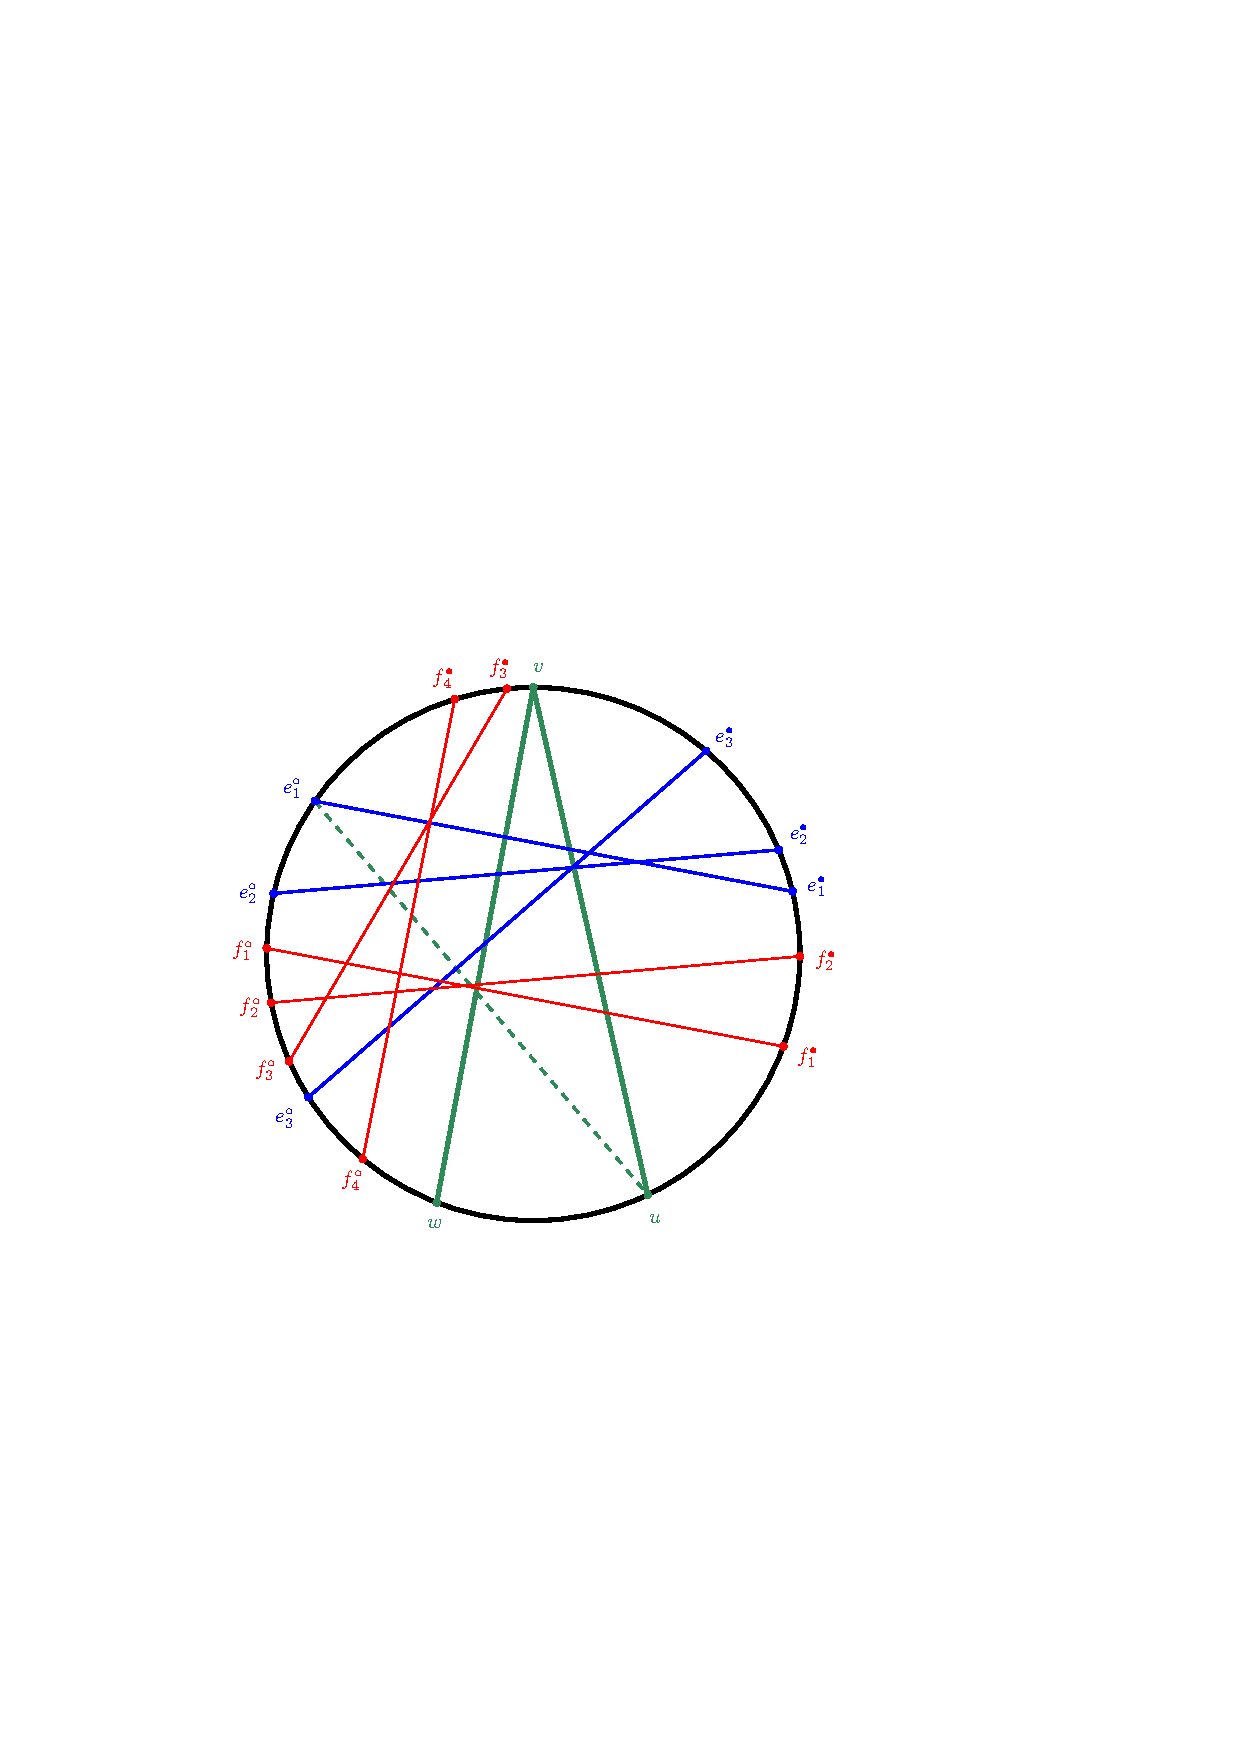
\includegraphics[width=\textwidth,page=1]{exProofStar}
  \end{subfigure}
  \begin{subfigure}[b]{.48\textwidth}
    \centering
    \includegraphics[width=\textwidth,page=2]{exProofStar}
  \end{subfigure}
  \caption{Illustrations of the first and second steps of the proof of \cref{prop:angleBelongStar}. In both case, $k=4$, and on the left, $\ell=2$.}
  \label{fig:exProofStar}
\end{figure}

\medskip
\paragraph{\bf First step.}
Suppose that $(u, e^\circ_1)$ is not in $T$. 
Since $T$ is a $k$-triangulation, there is a $k$-crossing $F=\{f_1, \dots, f_k\}$ (with $u \cl f^\bullet_1 \cl \cdots \cl f_k \cl e'_1 \cl f'_1 \cl \cdots \cl f'_k \cl u$) that prevents the diagonal~$(u, e^\circ_1)$. We will now exhibit a $(k-1)$-crossing of the form~$\{f_1, \dots, f_\ell, e_{\ell+1}, \dots, e_{k-1}\}$ that will cross~$\angle(u,v,w)$ and be $v$-farther than~$E$, contradicting the maximality of~$E$.

Note first that~$f^\bullet_k \in [v, e^\circ_1[$, as otherwise~$F \cup \{(u, v)\}$ would form a $(k + 1)$-crossing.
Additionnaly, $f^\circ_k \in {]e^\circ_1, w]}$, as otherwise $E \cup \{(v,w), (f^\bullet_k, f^\circ_k)\}$ would form a $(k + 1)$-crossing. 
Consequently, we have~$f^\circ_1 \in {]e^\circ_1, w[}$ $e^\circ_1 \cl f^\circ_1 \cl \cdots \cl f^\circ_{k-1} \cl w$.

Let $\ell = \max \set{j\in[k-1]}{\, f^\circ_i \in {]e^\circ_i, w[} \text{ for all } i \le j}$.
Then $f^\bullet_i \in {]u, e^\bullet_i]}$ for any $i \le \ell$, as otherwise $\{e_1, \dots , e_i, f_i, \dots , f_k\}$ would form a $(k + 1)$-crossing.
Thus~$f_i$ crosses~$\angle(u,v,w)$ and is $v$-farther than~$e_i$ for any~$i \le \ell$.
Furthermore, we have $f^\circ_\ell \cl f^\circ_{\ell+1} \cl e^\circ_{\ell+1}$ (by maximality of~$\ell$) and~$f^\bullet_\ell \cl e^\bullet_{\ell} \cl e^\bullet_{\ell+1}$, so that~$f_\ell$ crosses~
$e_{\ell+1}$. 
Consequently, we get a $(k-1)$-crossing $\{f_1, \dots , f_\ell, e_{\ell+1}, \dots , e_{k-1}\}$ which is $v$-farther than $\{e_1, \dots , e_{k-1}\}$, contradicting the maximality of~$E$. 
We conclude that~$(u, e^\circ_1)$ belongs to~$T$.

Suppose now that~$\angle(e^\bullet_1, e^\circ_1, u)$ is not an angle of~$T$. 
Then there exists $e^\bullet_0 \in {]u, e^\bullet_1[}$ such that $(e^\bullet_0, e^\circ_1) \in T$. 
But then the $(k-1)$-crossing $\{(e^\bullet_0, e^\circ_1), e_2, \dots, e_{k-1}\}$ is $v$-farther than~$E$. 
This implies that~$\angle(e^\bullet_1, e^\circ_1, u)$ is an angle of~$T$.

\medskip
\paragraph{\bf Second step.}
Assume now that there exists a $(k-1)$-crossing~$F=\{f_2, \dots , f_k\}$ that crosses $\angle(e^\bullet_1, e^\circ_1, u)$ and is $e^\circ_1$-farther than the $(k-1)$-crossing $\{e_2, \dots, e_{k-1}, (v, w)\}$.

Note first that~$f_k = (v,w)$. Indeed, since~$f_k$ is $e^\circ_1$-farther than~$(v,w)$, we have~$f^\bullet_k \in {]e^\bullet_1, v]}$ and~$f^\circ_k \in [w,u[$. Therefore~$f^\bullet_k = v$ (as otherwise~$\{(u,v), e_1\} \cup F$ would form a $(k+1)$-crossing), and~$f^\circ_k = w$ (since~$\angle(u,v,w)$ is an angle of~$T$).

Since~$f_k = (v,w)$, we obtain that~$\{e_1, f_2, \dots, f_{k-1}\}$ is a $(k-1)$-crossing that crosses~$\angle(u,v,w)$. For any $i \in [2,k-1]$, the diagonal~$f_i$ is $e^\circ_1$-farther than~$e_i$, and thus also $v$-farther than~$e_i$. Therefore, $\{e_1, f_2, \dots, f_{k-1}\}$ is $v$-farther than~$E$, contradicting the maximality of~$E$.
\end{proof}

Combining \cref{coro:farthestTidy} and \cref{prop:angleBelongStar}, we obtain the proof of \cref{thm:structureInfinite}\,(1):

\begin{corollary}
In a \ef \ktg of a tidy polygon, any $k$-relevant angle belongs to a $k$-star.
\end{corollary}

%%%%%%%%%%%%

\subsection{Any $k$-relevant diagonal belongs to $2$ $k$-stars, and can be flipped}

\begin{lemma}
When $k\geq 2$, any \ef \ktg of a \nbd is \vf.
\end{lemma}
\begin{proof}
Any diagonal of the $k$-border surrounding a given vertex intersects all diagonals adjacent to this vertex.
\end{proof}

\begin{lemma}
Any diagonal of a \vf \ktg belongs to $4$ angles.
\end{lemma}
\begin{proof}
The vertices adjacent to the diagonal have finite degree. Take the neighbours just before and after the other vertex. The $4$ hereby obtained diagonals form angles with the first one.
\end{proof}

\begin{lemma}
Any diagonal belongs to $2$ $k$-stars.
\end{lemma}
\begin{proof}
cf Pilaud Santos. to be adapted to the infinite case, but shouldn't need any additional hypothesis. quite long though : section 3.
\end{proof}

%%%%%%%%%%%%

\subsection{Flattening a boundary $k$-star, inflating a boundary $k$-crossing}

\begin{figure}
  \centering
  \begin{subfigure}[b]{.48\textwidth}
	\centering
	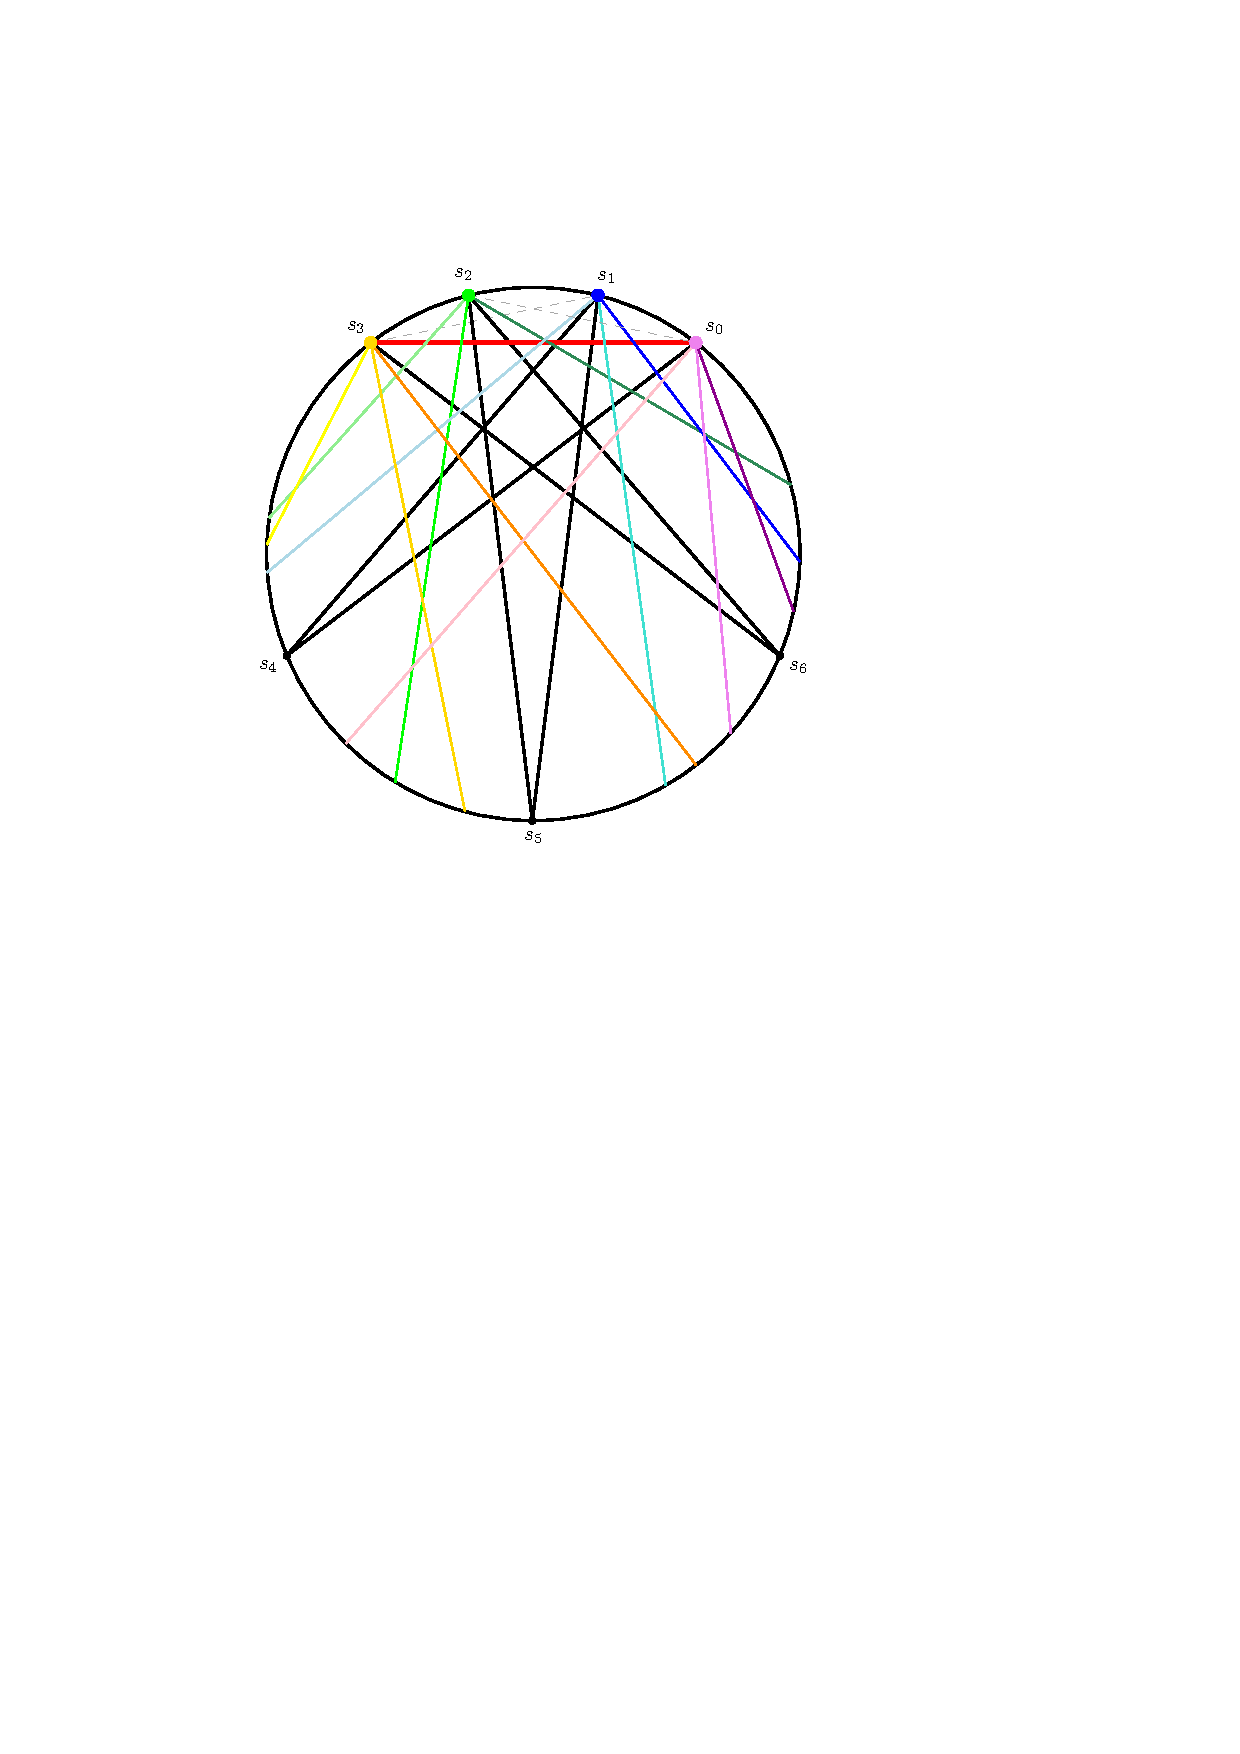
\includegraphics[width=\textwidth,page=1]{exFlattening}
  \end{subfigure}
  \begin{subfigure}[b]{.48\textwidth}
    \centering
    \includegraphics[width=\textwidth,page=2]{exFlattening}
  \end{subfigure}
  \caption{Illustrations of the flattening of a boundary $k$-star, with $k=3$.}
  \label{fig:exProofStar}
\end{figure}

%%%%%%%%%%%%%%%%%%%%%%%%%%%%%%%%%%%%%%

\section{multi-triangulations of the half-cylinder}

\begin{definition}
A \defn{half-cylinder} is a cylinder with no point on the upper border.
\end{definition}

%%%%%%%%%%%%

\subsection{Half-cylinder with $2$ marked points}

Consider the situation where the surface~$\surface$ is a cylinder with two points~$a,b$ on one boundary and none on the other.
\mathias{to be extended}
The universal cover is an infinite band, with points~$a_{\ell}, b_{\ell}$ for~$\ell \in \Z$ alternating on one boundary (so that~$a_\ell+1 = b_\ell = a_{\ell+1}-1$).
For~$k \ge 1$ and a word~$w \eqdef w^1 \dots w^k \eqdef  \in \{a,b\}^k$, consider a set~$T_w$ of diagonals of~$\surface$ formed by
\begin{itemize}
\item the diagonals~$(w^i_\ell, w^i_{\ell}+k+i)$ for all~$i \in [k]$ and~$\ell \in \Z$,
\item all $k$-boundary and $k$-irrelevant diagonals~$(\epsilon_{\ell}, \epsilon_{\ell}+i)$ for~$i \in [k]$, $\epsilon \in \{a,b\}$ and~$\ell \in \Z$.
%\item the outer $k$-boundary diagonals~$(a_{\ell}, a_{\ell}+2k)$ for~$\ell \in \Z$.
\end{itemize}
\vincent{Picture}

\begin{lemma}
\label{lem:noTwoDiagonalsEachLevel}
The sets
\begin{itemize}
\item $\set{(\epsilon_\ell, \epsilon_\ell+k+i)}{\epsilon \in \{a,b\} \text{ and } \ell \in \Z}$ for any~$i \in [k]$,
\item $\set{(\epsilon_\ell, \epsilon_\ell+k+i)}{\ell \in \Z}$ for any~$\epsilon \in \{a,b\}$ and~$i \ge k+1$,
\end{itemize}
all contain a $(k+1)$-crossing.
\end{lemma}

\begin{proposition}
For any~$k \ge 1$ and~$w \eqdef  \in \{a,b\}^k$, the set~$T_w$ is a $k$-triangulation of~$\surface$.
\end{proposition}

\begin{proof}
The maximality is immediate from \cref{lem:noTwoDiagonalsEachLevel}.
To see that~$T_w$ is $(k+1)$-crossing-free, we use the following strategy:
\begin{itemize}
\item the set of diagonals~$\set{(\epsilon_\ell, \epsilon_\ell+2k)}{\ell \in \Z}$ has no $(k+1)$-crossing for any~$\epsilon \in \{a,b\}$,
\item given any set~$X$ of pairwise crossing diagonals in~$T_w$, we can construct a new set~$X'$ of pairwise crossing diagonals in~$T_w$ by increasing the length of the smallest diagonal~$(u,v)$ of~$X$, provided this length is not~$2k$. Indeed, we just need to observe that the vertices~$u-1$ and~$v-1$ cannot be incident to diagonals of~$X$.
\qedhere
\end{itemize}
\end{proof}

\begin{corollary}
\label{coro:allkTriangCyclinder}
The set of $k$-triangulations of~$\surface$ is~$\set{T_w}{w \in \{a,b\}^k}$.
\end{corollary}

\begin{proof}
Any $(k+1)$-crossing free set of diagonals of~$\surface$ is a subset of a certain~$T_w$ by \cref{lem:noTwoDiagonalsEachLevel}.
\end{proof}

We denote by~$\delta_w^i$ the diagonal of~$\surface$ which lifts to the diagonals~$(w^i_\ell, w^i_{\ell}+k+1+i)$.

\begin{proposition}
%For any~$w \in \{a,b\}^k$ and~$i \in [k]$, the diagonal~$\delta_w^i$ of the $k$-triangulation~$T_w$ can be fli
For any~$w, w' \in \{a,b\}^k$ which only differ at position~$i \in [k]$, the $k$-triangulations~$T_w$ and~$T_w'$ are the only two $k$-triangulations~$\surface$ which contain~${T_w \ssm \{\delta_w^i\} = T_{w'} \ssm \{\delta_{w'}^i\}}$. In other words, any diagonal~$\delta_w^i$ in the $k$-triangulation~$T_w$ can be uniquely flipped.
\end{proposition}

\begin{proof}
By definition of~$T_w$ and~$T_{w'}$, we have~${T_w \ssm \{\delta_w^i\} = T_{w'} \ssm \{\delta_{w'}^i\}}$ so that the flip is possible.
It is unique by \cref{coro:allkTriangCyclinder}.
\end{proof}

\begin{remark}
The flip of $\delta_w^1$ is sequential (for the first flip, all points below $\delta_w^1$ are vertices of the star below~$\delta_w^1$ and we can determine which of these angles see each other; we have not worked out the other flips yet).
In contrast, the flip of~$\delta_w^i$ is not sequential for~$i \in \{2, \dots, k-1\}$ (since the common bisector is still of length~$k+1$).
\end{remark}

\begin{remark}
This is just an example of non-sequential flips on a cylinder. We need to understand all flips on a cylinder.
\end{remark}

%%%%%%%%%%%%

\subsection{Flips of a saturated multi-triangulation of a half-cylinder}

\begin{definition}
Let $T$ be a \ktg of the half-cylinder with $p$ points. We denote $n_T^l$ the number of edges of length $l$ in $T$. We say that $T$ is \defn{saturated} if there exists $L>k$ such that:
\begin{itemize}
\item $n_T^l=p$, for any $l\leq k$ (these are $k$-irrelevant and $k$-boundary edges),
\item $n_T^l=p-1$ for $l\in[k+1,L-1]$,
\item $n_T^l=0$ for $l>L.$ 
\end{itemize}
\end{definition}

\begin{theorem}
\label{thm:flipSaturated}
Any $k$-relevant edges of a saturated multi-triangulation of the half-cylinder can be flipped.
\end{theorem}

%%%%%%%%%%%%

\subsection{multi-triangulations of the half-cylinder with only one star}

\begin{theorem}\label{thm:uniStarSaturated}
Any multi-triangulation of a half-cylinder with only one star is saturated.
\end{theorem} 

Let $\mathcal{C}$ be a cylinder with $p$ points $(v_i)_{i\in\mathcal{Z}/p\mathcal{Z}}$ on one border and no point on the other border. Let $T$ be a $k$-triangulation of $\mathcal{C}$. Suppose $T$ only have $1$ $k$-star $S$.

The length of an edge of $T$ has to be greater or equal to $k$ ($k$-relevant) and smaller or equal to $pk$ (otherwise $k+1$ successive copies of this edges 
form a $k+1$-crossing).

We represent edges of $T$ as symbols on a square lattice.
Let $e$ be an edge of $T$. Suppose the left point of $e$ is $v_i$, and $e$ has length $l$. 
We define a symbol $\sigma(e)$ as being $\vee$ if $S$ is only on the upper side of $e$, $\wedge$ if it is only on the lower side, and $\times$ if it is on both sides.
Then $e$ is represented by the symbol $\sigma(e)$ at position $(i,l)$.
Additionally we add a symbol $\circ$ at every empty position which is directly under a symbol $\wedge$ or $\times$ and directly over a symbol $\vee$ or $\times$.
Note that this representation is entirely contained in a $p\times pk$ rectangle.

The star $S$ can be represented on the lattice by an excursion from symbol to symbol corresponding to a counter-clockwise tour of $S$.
In such a tour, whenever you reach an edge $(i,l)$ from an edge with smaller length, the next edge to follow is $(i,l')$ where $l'$ is the biggest length of an edge starting at vertex $v_i$, which is smaller than $l$.
Similarly, whenever you reach an edge $(i,l)$ from an edge with higher length, the next edge to follow is $(j,l')$ where $l'$ is the smallest length of an edge $(j,l')$ finishing at vertex $v_{i+l}$, which is bigger than $l$. In case there is no such edge, then you have to follow the edge $(i+l,l')$ where $l'$ is maximal (red edge).

By consequence the walk can be entirely deduced from the disposition of the points. see \cref{fig:exLattice}.

\begin{figure}\label{fig:exLattice}
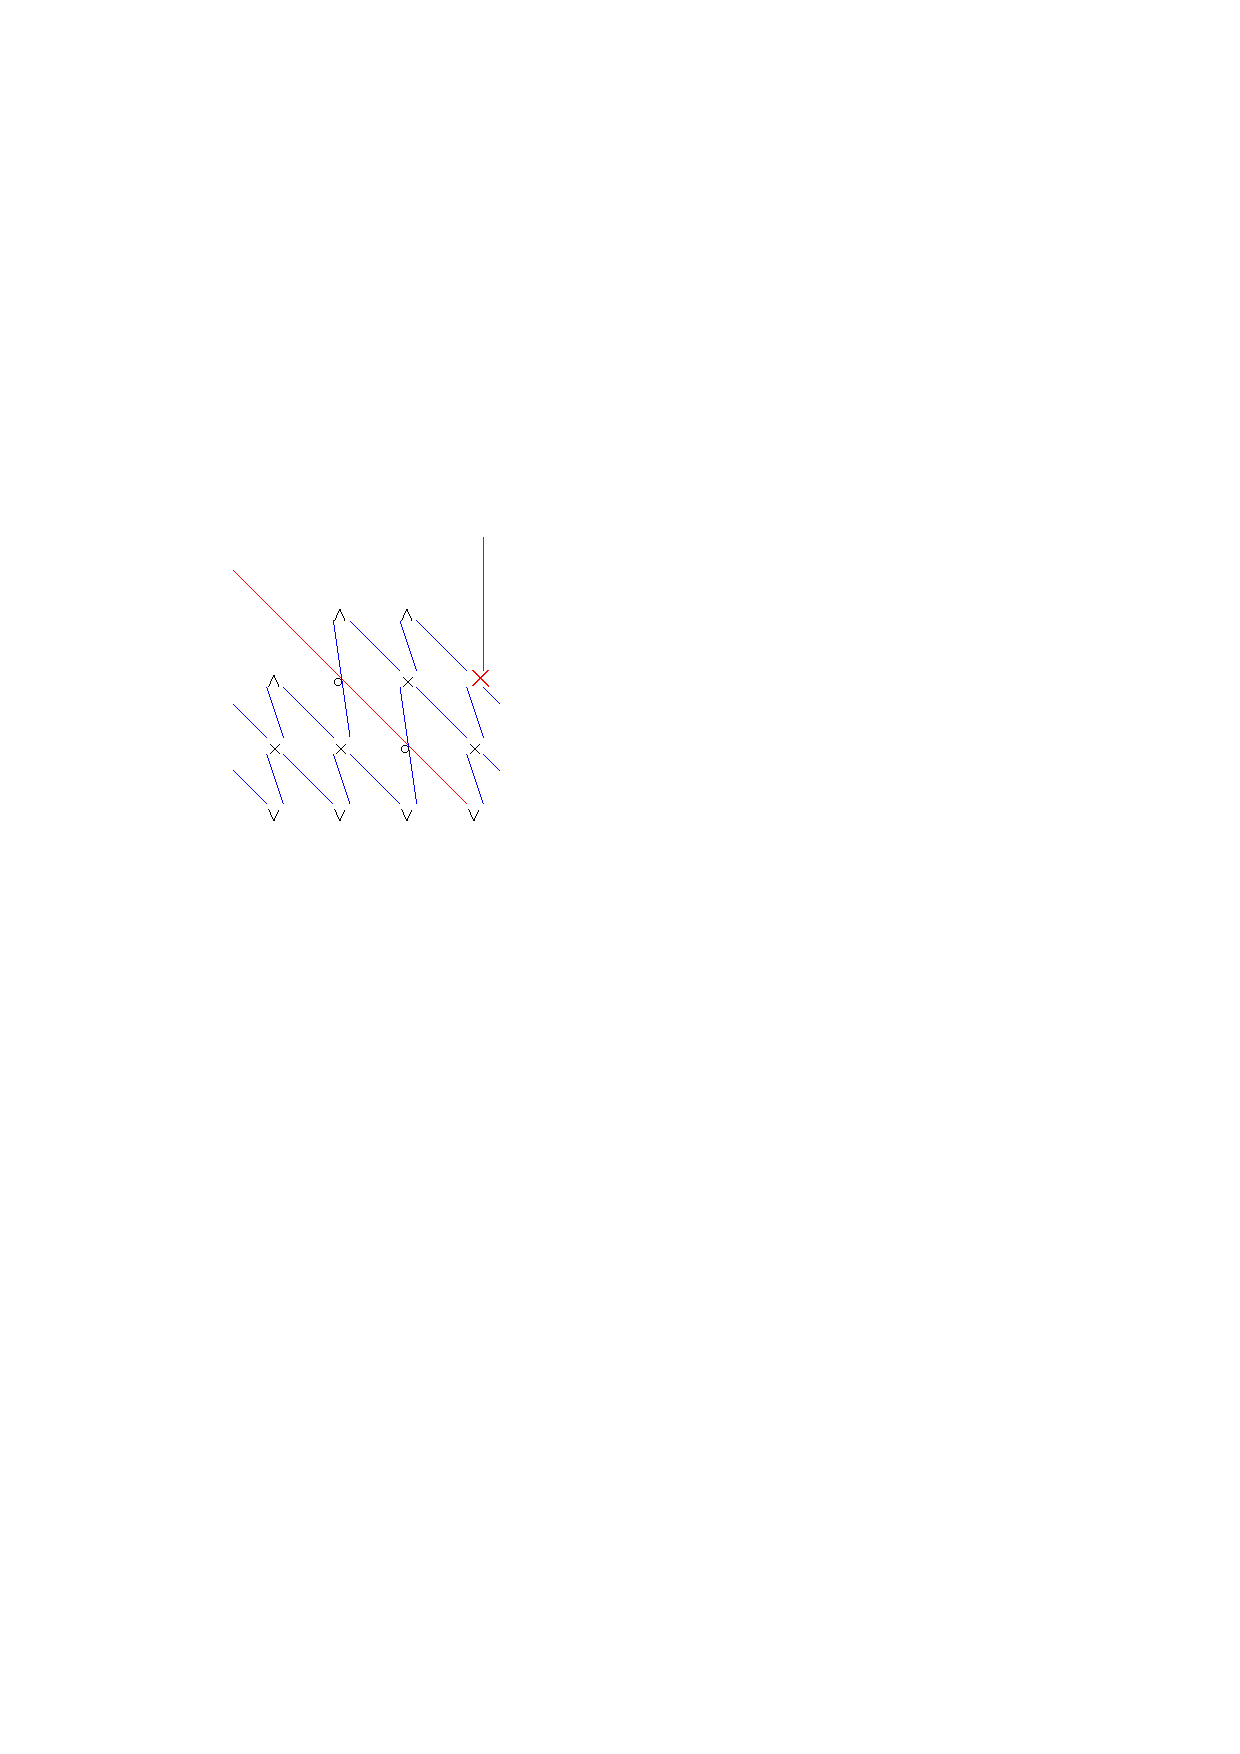
\includegraphics[width=.98\linewidth]{latticeRepresentation}
\caption{example of the lattice representation of $7$-triangulation with a unique star, on the half-cylinder with $4$ points.}
\end{figure}

%Since there is only one star, all $k$-border edges have to be part of the star. 
We denote $l_{min}$ and $l_{\max}$ the minimal and maximal length of an edge of $S$.

A $k$-star has $2k+1$ edges: $n_\vee+n_\wedge+2n_\times=2k+1$. It is on the upper side of $k+1$ of them and the lower side of $k$ of them: $n_\vee+n_\times=k+1$ and $n_\wedge+n_\times=k$.

We group edges by successive pairs: an edge followed by a smaller edge. This corresponds in the lattice to a vertical descending edge. Only the red edge remain unmatched. When doing a tour of $S$, each pair makes you go to the left by a length corresponding to the height of the corresponding vertical edge, and the edge corresponding to the red point makes you go to the right by a lenght corresponding to its length. In the end of the tour, you have to get back to your initial condition.

By consequence, the total length of blue vertical edges, denoted $\Delta$, has to be equal to the length of the edge corresponding to the red vertex, denoted $h$.

NB (to be proved): an excursion in the lattice corresponds to a $k$-star if and only if it has length $k+1$ and exactly $1$ red point/edge, and $\Delta=h$.


Over any symbol $\vee$, there is a sequence of $\circ$ and $\times$, ended by a $\wedge$ or a red $\times$ (and potentially followed by another sequence). Inside each of this sequence,  we know that all vertical edges are visited by the excursion. By consequence: $\Delta=n_\wedge+n_\times+n_\circ$. 

Let $l$ be a length such that $l_{min}<l<l_{max}$. Since the star is represented by a (connected) excursion, there exists a vertex $i$ such that $(i,l)$ has symbol $\circ$. By consequence, $n_\circ\geq l_{max}-l_{min}-1$.

By unicity of the red $\times$, the symbol coming just after the red $\times$ has to have length strictly bigger. By consequence $h<L$.  Note also that $l_{min}\geq k$.

By grouping everything together we obtain:

\begin{align}
0&=\Delta-h \\
&=n_\wedge+n_\times+n_\circ-h\\
&=k+n_\circ-h\\
&=(k-l_{min})+(l_{min}+n_\circ-l_{max}+1)+(l_{max}-1-h)
\end{align}

$k-l_{min}$ EST À L'ENVERS...  

By consequence: $l_{min}=k$, $n_\circ=L-k-1$ and $h=L-1$.

We showed that at each level between $k+1$ and $h$, there is exactly one point where the blue line goes through vertically. We can show in the exact same way that there is exactly one point where the blue line goes through diagonally.

If we count the special edge, each star has exactly $1$ vertical edge and 1 diagonal edge at all level $l>k$.


Note that we did not use the fact that the star is unique, so that this is true for any star of a triangulation of the half-cylinder. In particular, the number of star of such a triangulation is strictly smaller than $p$. see \cref{fig:2stars}.


\begin{figure}\label{fig:2stars}
\includegraphics[width=.98\linewidth,page=3]{latticeRepresentation}
\caption{an example of a $2$-triangulation of t	he half cylinder with $2$ points and $2$ stars.}
\end{figure}

\medskip

NOT TRUE ANYMORE, BECAUSE THEY ARE NOT $K$-TRIANGULATIONS (see ultrafat edges on picture) ET D'AILLEURS L_MAX>KP.
However it may be that there are more than $k$ $\vee$. See \cref{fig:problem}. The first line should be the smallest such configuration. However it has no flippable edge, unlike the second one. In the second configuration, it is still easy to flip the unique flippable edge. As always, it suffices to exchange a blue crossing with a $\circ$ (as illustrated in the second row of \cref{fig:problem}). 

\begin{figure}\label{fig:problem}
\includegraphics[width=.98\linewidth,page=2]{latticeRepresentation}
\caption{problems may occur...}
\end{figure}

%%%%%%%%%%%%

\subsection{Non-sequential flips and restriction to the cylinder}

Consider a $k$-triangulation~$T$ of a surface~$\surface$.
Let~$\bar T$ be the corresponding infinite $k$-triangulation of the universal cover~$\bar \surface$.
We want to show that any $k$-relevant arc~$\alpha$ of~$T$ is flippable.
The natural idea is to flip sequentially all copies~$\bar\alpha$ of the arc~$\alpha$ in~$\bar T$.
However, this only works if, at any point of this procedure, the flip of any copy~$\bar\alpha$ in~$\bar T$ does not modify the flip of the other copies of~$\alpha$ in~$\bar T$.
We say that the flip of~$\alpha$ in~$T$ is \defn{sequential} when this procedure works, and \defn{non-sequential} otherwise.

\begin{example}
A non sequential flip.
\end{example}


The goal of this section is to show that non-sequential flips in $k$-triangulations of any surface~$\surface$ just boil down to non-sequential flips of $k$-triangulations of a cylinder~$\cylinder$.
For this, consider an arc~$\alpha$ of a $k$-triangulation~$T$ of~$\surface$, and let~$S,S'$ be the two $k$-stars of~$T$ containing~$\alpha$.
We distinguish three cases:\mathias{3?}
\begin{itemize}
\item If~$S$ and~$S'$ are distinct $k$-stars of~$T$, then $\alpha$ appears only once in~$S$ and in~$S'$. Consider a copy~$\bar\alpha$ of~$\alpha$ in~$\bar T$ and the copy~$\bar S$ (resp.~$\bar S'$) of~$S$ (resp.~$S'$) in~$\bar T$ containing~$\bar\alpha$. Remember from \cref{sec:infiniteMultitriangulations} that the flip of~$\bar\alpha$ in~$\bar T$ only depends on and only modifies the two $k$-stars~$\bar S$ and~$\bar S'$. Since~$\bar\alpha$ is not contained in any other copy of~$S$ and~$S'$ in~$\bar T$, the flip of~$\bar\alpha$ in~$\bar T$ does not modify the flip of the other copies of~$\alpha$ in~$\bar T$. Therefore the flip is sequential.
\item Assume now that~$S = S'$ so that~$\alpha$ appears twice in~$S$. Let~$\bar\alpha$ and~$\bar\alpha'$ be two copies of~$\alpha$ in a copy~$\bar S$ of~$S$ in~$\bar T$. Let~$\pi$ be the homomorphism of~$\bar\surface$ such that~$\pi(\bar\alpha) = \bar\alpha'$. We consider the collection~$\bar U$ of arcs of stars~$\pi^i(\bar S)$ for~$i \in \Z$. Perform all identifications of two consecutive vertices of~$\bar U$ that do not uncross any pairs of arcs of~$\bar U$. These identifications can be performed in any order. The result~$\bar V$ is a $k$-triangulation of an infinite polygon whose homomorphism group is generated by~$\pi$. Therefore, $\bar V$ is a covering of a $k$-triangulation~$V$ of a cylinder~$\cylinder$.
\end{itemize}

\begin{theorem}
\label{thm:decompCylinder}
The surface obtained this way is a half-cylinder.
\end{theorem}

Combined with \cref{thm:flipSaturated,thm:uniStarSaturated}, we obtain \cref{generalFlip}.






\bibliographystyle{abbrv}
\bibliography{../bibliography}

\end{document}
